% 原書PDF99--112（本文77--90頁）、第3章導入および3.1--3.3。
\sectionlink{Polyakov経路積分}\label{ch:3}
\suppressfloats[t]

ここからは、Polyakov経路積分と共形場理論を用いて、弦理論を体系的に研究する。
経路積分の描像を導入したのち、ゲージ固定、Weyl異常、頂点演算子を議論する。
続いて、曲がった時空を伝播する弦へと一般化する。

\subsectionlink{世界面についての和}\label{sec:3.1}

Feynman経路積分は、量子論を表す一つの方法であり、
弦理論における相互作用を記述するうえで非常に自然な方法である。
経路積分量子化では、初期状態と終状態をつなぐ、
ありうるすべての履歴について和をとることで振幅を与える。
それぞれの履歴には
\begin{equation}
\exp(iS_{\mathrm{cl}}/\hbar)
\tag{3.1.1}\label{eq:3.1.1}
\end{equation}
という重みをつける。ここで、$S_{\mathrm{cl}}$はその履歴の古典作用である。
したがって、弦理論の振幅は、与えられた初期曲線と終曲線をつなぐすべての世界面に
ついて和をとることによって定義することになる。
開弦の場合を図\ref{fig:3.1}(a)、閉弦の場合を図\ref{fig:3.1}(b)に示す。
相対論的な点粒子について同様の和をとると、自由伝播関数が得られる（演習5.1）。

\begin{figure}[htbp]
\centering
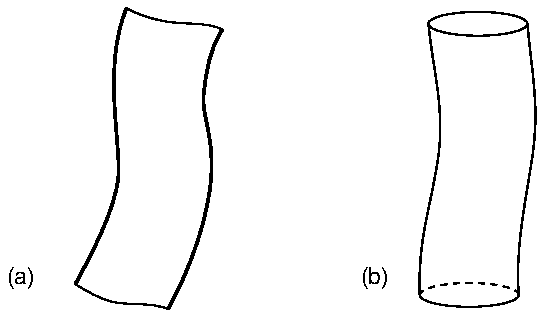
\includegraphics[width=0.82\linewidth]{figures/fig_3_1.pdf}
\caption{(a) 帯の位相を持つ開弦の世界面。太い曲線は弦の端点の世界線である。
(b) 円筒の位相を持つ閉弦の世界面。}
\label{fig:3.1}
\end{figure}

弦が相互作用する仕方はいくつも考えられる。
一つは、2本の弦が交差するときにエネルギーが生じる接触相互作用である。
もう一つは、何らかの量子場が媒介する長距離力である。
しかし、そのような相互作用を、対称性と整合するように弦理論に
\emph{付け加える}ことはできない。
なぜそうなのかについては、後である程度の理解を得ることになる。
許される相互作用は、世界面についての和にすでに暗黙に含まれているものだけである。
たとえば図\ref{fig:3.2}の世界面を考えよう。
図\ref{fig:3.2}(a)は、図\ref{fig:3.1}(a)の開弦振幅への量子補正のように見え、
2本の開弦からなる中間状態を含んでいる。
図\ref{fig:3.2}(b)には3本の外線の閉弦があり、1本の弦が2本に崩壊する過程を表している。
これこそが弦理論に相互作用を導入する正しい方法であることがわかる。
これらの相互作用が、有限でユニタリーであり、重力を含む整合的な理論を生み出すことを見るであろう。

\begin{figure}[tbp]
\centering
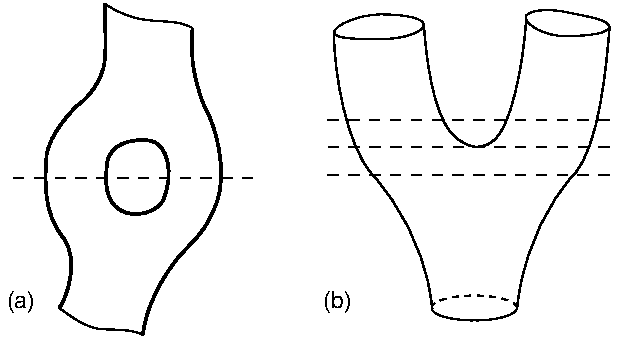
\includegraphics[width=0.86\linewidth]{figures/fig_3_2.pdf}
\caption{(a) 開弦の伝播への量子補正。(b) 1本の閉弦が2本に崩壊する過程。
破線は等時刻断面である。}
\label{fig:3.2}
\end{figure}

図\ref{fig:3.2}(b)の過程を、図\ref{fig:3.3}のように、
順々の時刻で観察してみると興味深い。
1本の閉弦が2本に分かれる。あるいは、その逆の過程では2本が1本につながる。
これが閉弦の基本的な相互作用である。
閉弦理論では、すべての粒子は弦のさまざまな励起状態として得られ、
すべての相互作用（たとえばゲージ相互作用、重力相互作用、Yukawa相互作用）は、
図\ref{fig:3.3}の一つの過程から生じる。
開弦を含む理論では、図\ref{fig:3.4}に示すように、
これに加えていくつかの過程が起こりうる。
ある時間分割を選ぶと、図\ref{fig:3.3}および図\ref{fig:3.4}の相互作用は
時空のある定まった点で起こるように見えるが、これは見かけにすぎない。
Lorentzブーストした座標系で別の時間分割を選ぶと、
見かけの相互作用は別の点に位置することになる。
時空に特別な点があるわけではない。
相互作用は世界面の大域的な位相だけから生じ、
世界面の局所的な性質は自由な場合と同じである。
序論で述べたように、このように相互作用が広がることによって、
重力の短距離発散が切り落とされる。

\begin{figure}[tbp]
\centering
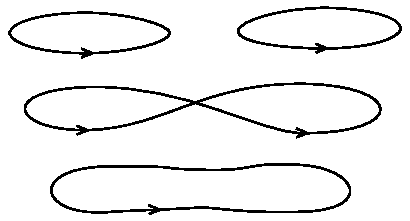
\includegraphics[width=0.67\linewidth]{figures/fig_3_3.pdf}
\caption{図\ref{fig:3.2}(b)の連続する等時刻断面。
矢印は弦の向きを表す。}
\label{fig:3.3}
\end{figure}

\begin{figure}[tbp]
\centering
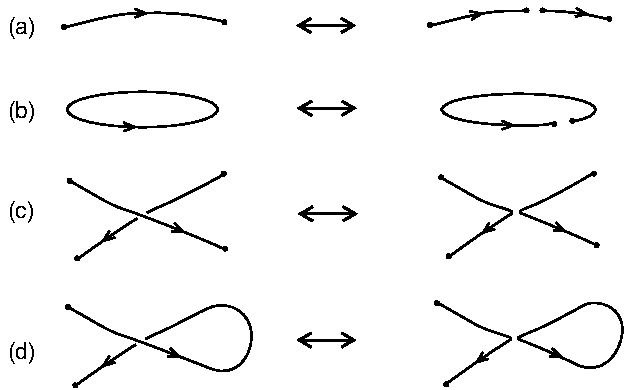
\includegraphics[width=0.84\linewidth]{figures/fig_3_4.pdf}
\caption{開弦を含む過程：
(a) 開弦$\leftrightarrow$開弦$+$開弦、
(b) 閉弦$\leftrightarrow$開弦、
(c) 開弦$+$開弦$\leftrightarrow$開弦$+$開弦、
(d) 開弦$\leftrightarrow$開弦$+$閉弦。}
\label{fig:3.4}
\end{figure}

実際には、世界面についての和にどの位相を含めるかによって、
いくつかの異なる弦理論が存在する。
まず、これまで描いてきた世界面には2種類の境界があることに注意しよう。
初期状態および終状態の弦の配位に対応する\emph{ソース境界}と、
開弦の端点の世界線に対応する\emph{端点境界}である。
ソース境界はひとまず無視しよう。
ソースの詳細については、この章の後のほうで議論する。
したがって、以下の議論で「境界」といえば端点境界を意味する。
すると、世界面についての和を定義する方法は次の4通りとなり、
これらは第1.4節の末尾に挙げた4種類の自由弦理論に対応する。
\begin{enumerate}
\item 向きのある閉弦：境界を持たない、向きのあるすべての世界面。
\item 向きのない閉弦：境界を持たないすべての世界面。
\item 向きのある閉弦と開弦：任意個数の境界を持つ、向きのあるすべての世界面。
\item 向きのない閉弦と開弦：任意個数の境界を持つすべての世界面。
\end{enumerate}

\begin{figure}[tbp]
\centering
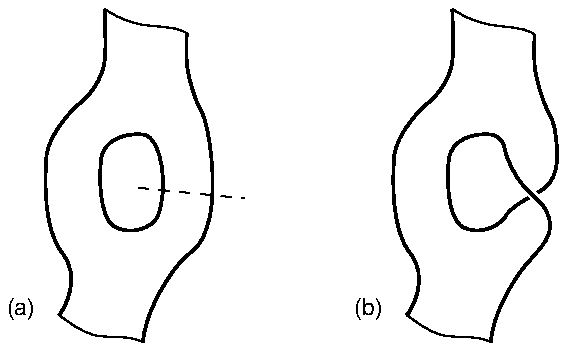
\includegraphics[width=0.80\linewidth]{figures/fig_3_5.pdf}
\caption{2本の開弦の振幅への、向きのある寄与(a)と向きのない寄与(b)。}
\label{fig:3.5}
\end{figure}

ここで、さらに説明すべきことが二つある。
第一は、向きのない世界面を含めることと、
第1.4節で説明した$\Omega=+1$への射影との関係である。
図\ref{fig:3.5}は、開弦を含む向きのない理論で和に含まれる二つの世界面を示している。
図\ref{fig:3.5}(b)の向きのない世界面は、
図\ref{fig:3.5}(a)の向きのある曲面を、$0\leq\sigma\leq\pi$で
パラメーター表示した破線に沿って切り、切り口上の場に
\begin{equation}
X^\mu_{\mathrm{upper}}(\sigma)
=X^\mu_{\mathrm{lower}}(\pi-\sigma)
\tag{3.1.2}\label{eq:3.1.2}
\end{equation}
を満たすことを要求するのと同等である。
これはさらに、開弦の状態に演算子$\Omega$を作用させることと同等である。
したがって、この二つの曲面を適切な重みで足し合わせることは、
$\Omega=+1$の状態へ射影する演算子$\frac12(1+\Omega)$を挿入することに相当する。
向きのある曲面と向きのない曲面のすべてについて和をとると、
すべての中間状態に射影演算子が挿入され、
スペクトルは$\Omega=+1$のセクターに制限される。

\begin{figure}[tbp]
\centering
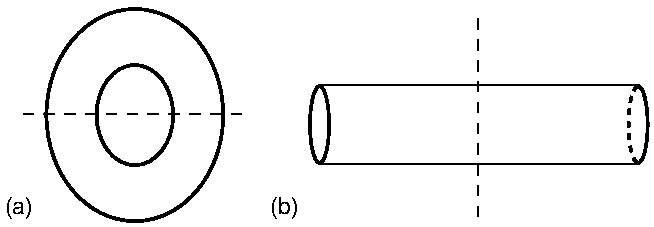
\includegraphics[width=0.90\linewidth]{figures/fig_3_6.pdf}
\caption{(a) 環帯：中間状態は2本の開弦からなる。
(b) 同じ位相を円筒として描いたもの：中間状態は1本の閉弦である。}
\label{fig:3.6}
\end{figure}

第二に、上の一覧には、開弦を持つが閉弦を持たない理論は含まれていない。
なぜそうなるのか、もう少し詳しく説明しよう。
図\ref{fig:3.6}(a)のように、環帯の位相を持つ世界面を考える。
便宜上、真空振幅だけを描いたが、
適切なソースをつなげれば同じ議論が散乱振幅にも適用できる。
破線からわかるように、これは2本の開弦からなる中間状態を持つ過程であり、
したがって、この位相の世界面は開弦を含むどの理論にも存在しなければならない。
図\ref{fig:3.6}(b)では、同じ位相を円筒として描き、
1本の閉弦からなる中間状態に沿って切り開いている。
したがって、開弦だけから出発したとしても、
世界面についての和には、開弦の散乱によって閉弦が生成される過程が必ず含まれる。
振幅を詳しく調べていく際に、これがどのように働くかを具体的に見ることになる。

開弦理論に閉弦が必要であることは、別の方法でも理解できる。
図\ref{fig:3.4}(a)、(b)の相互作用を、時間を逆にして考えよう。
それぞれ、2本の開弦が1本に結合する過程と、開弦から閉弦への遷移である。
相互作用点の近くでは、これらはどちらも二つの端点が合体する同じ過程である。
第二の相互作用を許さずに第一だけを許すには、
弦のダイナミクスに何らかの非局所的な制約を課す必要があるだろう。
これはきっと不整合になるはずである。
図\ref{fig:3.4}(c)、(d)についても同じ議論ができる。
そこでは、相互作用は局所的には一対の弦のつなぎ替えである。
したがって、開弦の相互作用を何か一つでも許せば、
開弦から閉弦を生成する過程も何かしら許されることになる。

\subsectionlink{Polyakov経路積分}\label{sec:3.2}

ここからは、Polyakovの形式の場について積分することで、
世界面についての和を具体的に組み立てていく。
第1章から一つ変更を加える。
Minkowski世界面計量$\gamma_{ab}$を、符号$(+,+)$の
Euclid世界面計量$g_{ab}(\sigma^1,\sigma^2)$で置き換えるのである。
積分は、すべてのEuclid計量と、
世界面のMinkowski時空へのすべての埋め込み$X^\mu(\sigma^1,\sigma^2)$にわたる。
\begin{equation}
\int[dX\,dg]\,\exp(-S).
\tag{3.2.1}\label{eq:3.2.1}
\end{equation}
Euclid作用は
\begin{equation}
S=S_X+\lambda\chi
\tag{3.2.2}\label{eq:3.2.2}
\end{equation}
であり、ここで
\begin{align}
S_X&=\frac{1}{4\pi\alpha'}\int_M d^2\sigma\,g^{1/2}g^{ab}
       \partial_aX^\mu\partial_bX_\mu,
\tag{3.2.3a}\label{eq:3.2.3a}\\
\chi&=\frac{1}{4\pi}\int_M d^2\sigma\,g^{1/2}R
       +\frac{1}{2\pi}\int_{\partial M}ds\,k.
\tag{3.2.3b}\label{eq:3.2.3b}
\end{align}
測地曲率$k$は演習1.3で定義した。
ここでは境界がつねに空間的であることに注意しよう。

Euclid経路積分の利点は、計量についての積分がより明確に定義されることにある。
これまで説明してきた位相的に非自明な世界面は、
非特異なEuclid計量を持ちうるが、非特異なMinkowski計量を持つことはできない。
本書ではEuclid理論\eqref{eq:3.2.1}を出発点とし、
それに厳密な定義を与える方法と、それがこれまで述べてきた性質を備える
整合的な時空の理論を定義することを示す。
しかし、その前に、これが最初に出発したMinkowski理論と等価であることを、
簡単な形式的議論によって示しておこう。

再び点粒子の例から始める。この場合、経路積分
\begin{equation}
\int[d\eta\,dX]\,
\exp\left[\frac{i}{2}\int d\tau
\left(\eta^{-1}\dot X^\mu\dot X_\mu-\eta m^2\right)\right]
\tag{3.2.4}\label{eq:3.2.4}
\end{equation}
は振動的である。
$\eta$と$X^\mu$についての経路積分は通常の積分の積であるから、
通常の積分と同様に積分路を変形することができる。
無限小の$\theta$に対して
\begin{equation}
\eta(\tau)\longrightarrow e^{-i\theta}\eta(\tau),\qquad
X^0(\tau)\longrightarrow e^{-i\theta}X^0(\tau)
\tag{3.2.5}\label{eq:3.2.5}
\end{equation}
とすると、指数の中のすべての項に負の実部が加わるため、
これは収束因子として働く。
そこで、場の空間で積分路の回転を行い、
$\eta=-ie$、$X^0=-iX^D$まで回すことができる。
積分は
\begin{equation}
\int[de\,dX]\,
\exp\left[-\frac12\int d\tau
\left(e^{-1}\sum_{\mu=1}^{D}\dot X^\mu\dot X^\mu+em^2\right)\right]
\tag{3.2.6}\label{eq:3.2.6}
\end{equation}
となる。
これは経路積分\eqref{eq:3.2.1}に対応する、Euclid点粒子の場合の式である。
行ったのは積分路の回転だけなので、Euclid経路積分はMinkowski経路積分と
同じ振幅を与える。

Polyakov作用についても、計量を四脚場を用いて
$\gamma_{ab}=-e_a^0e_b^0+e_a^1e_b^1$と書き、
$e_a^0$に対して同じ回転を行えば、同じ手順が使える。
これによって、Minkowski経路積分とEuclid経路積分の等価性が形式的に正当化される。
\footnote[1]{2次元より高い次元では、Hilbert作用が回転のもとで
より複雑に振る舞うため、事情はそれほど簡単ではない。
経路積分を減衰させる単純な回転は存在しない。
特に、4次元重力のEuclid経路積分が何を意味するかは、非常に不確かである。}
両者をそれぞれ光円錐ゲージと共形ゲージで扱うと同じ振幅が定義されることが、
具体的な計算によって示されている。
作用\eqref{eq:3.2.3a}では、時空がMinkowski的であることを強調するために、
前章と同様、$X^0$の回転を暗黙のままにしておいた。
$X^0$を用いて書けば、運動方程式とOPEは計量$\eta^{\mu\nu}$に関して共変である。

$\chi$が2次元では局所的に全微分であり、
そのため世界面の位相だけに依存することは、すでに述べた。
これは世界面の\emph{Euler数}である。
したがって、経路積分における$e^{-\lambda\chi}$という因子は、
世界面についての和の中で、異なる位相の相対的な重みだけに影響する。
特に、図\ref{fig:3.1}(a)から図\ref{fig:3.2}(a)へ移る際に行ったように、
世界面に帯を一つ付け加えると、Euler数が1だけ減少し、
経路積分には$e^\lambda$という重みの因子が余分に掛かる。
帯を加えることは仮想的な開弦の放出と再吸収に対応するので、
どの過程からであっても、開弦を放出する振幅は$e^{\lambda/2}$に比例する。
任意の世界面に取っ手を一つ付け加えると、
Euler数が2だけ減少し、$e^{2\lambda}$という因子が掛かる。
これは閉弦の放出と再吸収に対応するので、
閉弦を放出する振幅は$e^\lambda$に比例する。
したがって、作用のEuler項が弦理論の結合定数を制御し、
\begin{equation}
g_{\mathrm o}^{\,2}\sim g_{\mathrm c}\sim e^\lambda
\tag{3.2.7}\label{eq:3.2.7}
\end{equation}
となる。
ところで、$\lambda$は理論の自由なパラメーターのように見えるかもしれない。
すると、弦理論にはそのようなパラメーターが存在しないという序論の主張と矛盾する。
これは重要な点であり、第3.7節で解決する。

余談になるが、結合定数の数え上げは、
弦のソースを持つ世界面にも単純な形で拡張できる。
閉弦のソースは閉じた境界ループであり、開弦のソースは境界の一部分である。
便宜上、開弦のソース境界が世界面計量に関して直角に端点境界と交わることを要求する。
角では境界曲率$k$が発散するので注意しなければならない。
Euler数は
\begin{equation}
\chi=\tilde\chi+\frac14n_{\mathrm c}
\tag{3.2.8}\label{eq:3.2.8}
\end{equation}
である。ここで、$\tilde\chi$には境界の滑らかな部分に沿った積分だけを含め、
$n_{\mathrm c}$は角の個数を表す。
経路積分に対する正しい重みは
\begin{equation}
\exp(-\lambda\tilde\chi)=\exp(-\lambda\chi+\lambda n_{\mathrm c}/4)
\tag{3.2.9}\label{eq:3.2.9}
\end{equation}
である。
これはユニタリティから従う。
世界面を切って内部線を減らし、外部ソースを増やしても、
$\lambda$依存性は変わってはならない。
$\tilde\chi$に含まれる表面積分が切り口で相殺するため、
重み\eqref{eq:3.2.9}ならばこの条件が満たされる。
閉弦のソースを加えることは世界面に穴を開けることに相当し、
$\chi$を1だけ減少させる。
開弦のソースを加えても$\chi$は変わらず、$n_{\mathrm c}$が2だけ増加する。
したがって、閉弦または開弦を放出する振幅について、
同じ結論\eqref{eq:3.2.7}に到達する。

\subsectionlink{ゲージ固定}\label{sec:3.3}

経路積分\eqref{eq:3.2.1}は、完全には正しくない。
そこには膨大な重複計数が含まれている。
局所的な$\mathrm{diff}\times\mathrm{Weyl}$対称性によって互いに関係する
配位$(X,g)$と$(X',g')$は、同じ物理的配位を表すからである。
実質的には、この局所対称群の体積で割る必要がある。
\begin{equation}
\int\frac{[dX\,dg]}{V_{\mathrm{diff}\times\mathrm{Weyl}}}\,\exp(-S)
\equiv Z.
\tag{3.3.1}\label{eq:3.3.1}
\end{equation}
これをゲージ固定によって行う。
すなわち、各ゲージ同値類を1回ずつ横切る断面に沿って積分し、
その断面上の正しい測度をFaddeev--Popov法によって求める。

第1章では光円錐ゲージを課した。
これはある目的には有用だが、理論の対称性の一部を隠してしまうので、
ここでは別の選び方をする。
計量は対称なので三つの独立な成分を持つこと、
そして、二つの座標と計量の局所的なスケールという、
三つのゲージ関数があることに注意しよう。
したがって、計量についての積分を消去し、
ある特定の関数形に固定するのにちょうど十分なゲージ自由度がある。
この固定した計量を\emph{基準計量}と呼び、
\begin{equation}
g_{ab}(\sigma)\longrightarrow\hat g_{ab}(\sigma)
\tag{3.3.2}\label{eq:3.3.2}
\end{equation}
と書く。
単純な選択は、平坦な計量、すなわち\emph{単位ゲージ}の計量
\begin{equation}
\hat g_{ab}(\sigma)=\delta_{ab}
\tag{3.3.3}\label{eq:3.3.3}
\end{equation}
である。
場合によっては、$\mathrm{diff}$群だけの効果を考えたいこともある。
その場合、任意の計量を、単位計量とWeyl変換だけ異なる形にすることができる。
これが\emph{共形ゲージ}である。
\begin{equation}
\hat g_{ab}(\sigma)=\exp[2\omega(\sigma)]\delta_{ab}.
\tag{3.3.4}\label{eq:3.3.4}
\end{equation}

場とゲージ対称性のこの数え上げが実際にうまくいくこと、
つまり、任意の計量を、少なくとも局所的に、
世界面上のある近傍では平坦な形にできることを具体的に見よう。
まずWeyl変換を行い、$g_{ab}$から作られるRicciスカラーをゼロにする。
RicciスカラーのWeyl変換は
\begin{equation}
g'^{\,1/2}R'=g^{1/2}(R-2\nabla^2\omega)
\tag{3.3.5}\label{eq:3.3.5}
\end{equation}
である。
$R'=0$とするには、$2\nabla^2\omega=R$を$\omega$に関する方程式として解く必要がある。
静電気学の標準的な議論により、これは少なくとも局所的にはつねに可能である。
さて、2次元ではRicciスカラーがゼロになることは、
Riemannテンソル全体がゼロになることを意味する。
Riemannテンソルの対称性から
\begin{equation}
R_{abcd}=\frac12(g_{ac}g_{bd}-g_{ad}g_{bc})R
\tag{3.3.6}\label{eq:3.3.6}
\end{equation}
が従うからである。
したがって、計量は平坦であり、座標変換によって単位計量\eqref{eq:3.3.3}と同等になる。

実際には、局所的には少し余分なゲージ自由度が残っている。
計量を単位ゲージのままに保つ$\mathrm{diff}\times\mathrm{Weyl}$変換が存在し、
これは計量の選択によっては固定されない。
ここでは、第2章と同じく複素座標$z=\sigma^1+i\sigma^2$を導入すると便利である。
この座標では平坦な計量は$ds^2=dz\,d\bar z$となる。
$z'$が$z$の正則関数となる座標変換
\begin{equation}
z'\equiv\sigma'^{\,1}+i\sigma'^{\,2}=f(z)
\tag{3.3.7}\label{eq:3.3.7}
\end{equation}
と、Weyl変換とを組み合わせて考える。
新しい計量は
\begin{equation}
ds'^{\,2}=\exp(2\omega)|\partial_zf|^{-2}\,dz'\,d\bar z'
\tag{3.3.8}\label{eq:3.3.8}
\end{equation}
である。
したがって、
\begin{equation}
\omega=\ln|\partial_zf|
\tag{3.3.9}\label{eq:3.3.9}
\end{equation}
ならば計量は不変である。
この余分なゲージ自由度は、先ほどの数え上げ（$3=3$）とは矛盾しない。
その食い違いに当たる正則な再パラメーター化の集合は、
すべての再パラメーター化の集合に比べれば測度ゼロだからである。

世界面全体を考えると、この余分な自由度のほとんど、またはすべては境界条件によって取り除かれる。
ここには二つの論点がある。
第一に、Noetherの定理とWard恒等式を議論した際、
式\eqref{eq:2.3.10}の下で、これらの結果は、
対称性が世界面上で局所的に定義されることだけに依存すると注意深く強調した。
したがって、変換\eqref{eq:3.3.7}、\eqref{eq:3.3.9}は、
保存カレントとWard恒等式をもたらす。
これは、まさに第2章で研究した共形不変性である。
それが、単位計量を不変に保つ$\mathrm{diff}\times\mathrm{Weyl}$の部分群として
現れることがわかる。

第二の論点は、世界面全体を考えたとき、
計量とゲージの自由度の数え上げがどうなるかである。
これは第5章で取り上げる。
そこで、大域的には両者の間に、有限個のパラメーターという小さな食い違いがあることを見る。
それまでは、世界面理論の局所的性質だけを扱うことにする。

\subsubsectionlink*{Faddeev--Popov行列式}

計量を固定すると、汎関数積分は$X^\mu$だけでパラメーター表示される断面に沿ったものとなる。
正しい測度を得るために、Faddeev--Popovの手順に従う。
手順は、Yang--Mills理論でゲージ固定された測度を得るために用いるものと同じだが、
ここでは自己完結した説明を与える。
図\ref{fig:3.7}に示すその考え方は、
経路積分をゲージ群についての積分とゲージ断面に沿った積分との積に分離し、
前者で割るというものである。
Faddeev--Popov行列式は、この変数変換のJacobianである。

\begin{figure}[tbp]
\centering
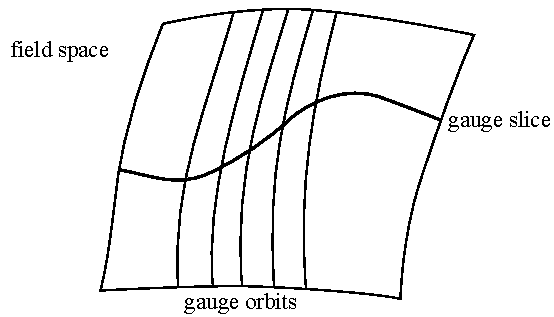
\includegraphics[width=0.84\linewidth]{figures/fig_3_7.pdf}
\caption{Faddeev--Popovの手順の模式図。
ゲージ軌道は、ゲージ同値な配位からなる族である。
場の空間全体について積分して軌道の体積で割ることは、
各軌道と1回ずつ交わる断面について、適切なJacobianを伴って積分することと同等である。
図中のfield spaceは場の空間、gauge sliceはゲージ断面、
gauge orbitsはゲージ軌道を表す。}
\label{fig:3.7}
\end{figure}

座標変換とWeyl変換を組み合わせた変換を、略して$\zeta$と書こう。
\begin{equation}
\zeta:g\longrightarrow g^\zeta,\qquad
g^\zeta_{ab}(\sigma')
=\exp[2\omega(\sigma)]
\frac{\partial\sigma^c}{\partial\sigma'^{\,a}}
\frac{\partial\sigma^d}{\partial\sigma'^{\,b}}g_{cd}(\sigma).
\tag{3.3.10}\label{eq:3.3.10}
\end{equation}
標準的な道筋に従い、Faddeev--Popov測度$\Delta_{\mathrm{FP}}$を
\begin{equation}
1=\Delta_{\mathrm{FP}}(g)\int[d\zeta]\,\delta(g-\hat g^\zeta)
\tag{3.3.11}\label{eq:3.3.11}
\end{equation}
によって定義する。ここでも$\hat g_{ab}$は基準計量である。
式\eqref{eq:3.3.11}の$[d\zeta]$は、
$\mathrm{diff}\times\mathrm{Weyl}$群上のゲージ不変な測度である。
この測度の具体的な形は必要にならない。
その存在の問題については次節で議論する。
デルタ関数は実際にはデルタ汎関数であり、
各点で$g_{ab}(\sigma)=\hat g^\zeta_{ab}(\sigma)$であることを要求している。

\eqref{eq:3.3.11}を汎関数積分\eqref{eq:3.3.1}に挿入すると、
後者は
\begin{equation}
Z[\hat g]
=\int\frac{[d\zeta\,dX\,dg]}{V_{\mathrm{diff}\times\mathrm{Weyl}}}
\Delta_{\mathrm{FP}}(g)\delta(g-\hat g^\zeta)\exp(-S[X,g])
\tag{3.3.12}\label{eq:3.3.12}
\end{equation}
となる。
後で参照するために、基準計量の選択に対する$Z$の依存性を明示しておく。
$g_{ab}$について積分を実行し、さらに積分変数の名前を$X\to X^\zeta$と変えると、
\begin{equation}
Z[\hat g]
=\int\frac{[d\zeta\,dX^\zeta]}{V_{\mathrm{diff}\times\mathrm{Weyl}}}
\Delta_{\mathrm{FP}}(\hat g^\zeta)\exp(-S[X^\zeta,\hat g^\zeta])
\tag{3.3.13}\label{eq:3.3.13}
\end{equation}
を得る。
ここで、$\Delta_{\mathrm{FP}}$、汎関数積分の測度$[dX]$、
作用のゲージ不変性を用いると、\footnote[2]{この不変性は次のように示せる。
\[
\begin{aligned}
\Delta_{\mathrm{FP}}(g^\zeta)^{-1}
&=\int[d\zeta']\,\delta(g^\zeta-\hat g^{\zeta'})\\
&=\int[d\zeta']\,\delta(g-\hat g^{\zeta^{-1}\cdot\zeta'})\\
&=\int[d\zeta'']\,\delta(g-\hat g^{\zeta''})
=\Delta_{\mathrm{FP}}(g)^{-1}.
\end{aligned}
\]
ここで$\zeta''=\zeta^{-1}\cdot\zeta'$である。
第2の等号ではデルタ関数のゲージ不変性を、
第3の等号では測度の不変性を用いた。}
\begin{equation}
Z[\hat g]
=\int\frac{[d\zeta\,dX]}{V_{\mathrm{diff}\times\mathrm{Weyl}}}
\Delta_{\mathrm{FP}}(\hat g)\exp(-S[X,\hat g])
\tag{3.3.14}\label{eq:3.3.14}
\end{equation}
となる。
最後に、被積分関数には$\zeta$に依存するものが何もないので、
$\zeta$についての積分は単にゲージ群の体積を与え、分母を打ち消す。
したがって、
\begin{equation}
Z[\hat g]=\int[dX]\,\Delta_{\mathrm{FP}}(\hat g)\exp(-S[X,\hat g])
\tag{3.3.15}\label{eq:3.3.15}
\end{equation}
が残る。このように、$\Delta_{\mathrm{FP}}(\hat g)$は断面上の正しい測度である。

Faddeev--Popov測度の表式\eqref{eq:3.3.11}を評価するために、
ゲージの選択がゲージ対称性をちょうど完全に固定すると仮定してみよう。
すなわち、デルタ関数$\delta(g-\hat g^\zeta)$がゼロでないのは、
厳密に一つの$\zeta$に対してだけであるとする。
$\delta(\hat g-\hat g^\zeta)$の場合には、それは恒等変換である。
上で述べたように、大域的には小さな食い違いがあるが、
それは必要になったときに扱うことにする。
世界面の局所的性質には影響しないからである。
$\zeta$が恒等変換に近いとき、
\begin{equation}
\begin{aligned}
\delta g_{ab}
&=2\delta\omega\,g_{ab}-\nabla_a\delta\sigma_b-\nabla_b\delta\sigma_a\\
&=(2\delta\omega-\nabla_c\delta\sigma^c)g_{ab}
   -2(P_1\delta\sigma)_{ab}
\end{aligned}
\tag{3.3.16}\label{eq:3.3.16}
\end{equation}
と展開できる。
ここでは、ベクトルをトレースのない対称2階テンソルへ写す微分演算子$P_1$を
\begin{equation}
(P_1\delta\sigma)_{ab}
=\frac12\left(\nabla_a\delta\sigma_b+\nabla_b\delta\sigma_a
             -g_{ab}\nabla_c\delta\sigma^c\right)
\tag{3.3.17}\label{eq:3.3.17}
\end{equation}
と定義した。
恒等変換の近傍では、逆行列式\eqref{eq:3.3.11}は
\begin{equation}
\begin{aligned}
&\Delta_{\mathrm{FP}}(\hat g)^{-1}\\
&\quad=\int[d\delta\omega\,d\delta\sigma]\,
 \delta\left[-(2\delta\omega-\hat\nabla\cdot\delta\sigma)\hat g
                    +2\hat P_1\delta\sigma\right]\\
&\quad=\int[d\delta\omega\,d\beta\,d\delta\sigma]\,
 \exp\biggl\{2\pi i\int d^2\sigma\,\hat g^{1/2}\beta^{ab}\\
&\hspace{37mm}\times
 \left[-(2\delta\omega-\hat\nabla\cdot\delta\sigma)\hat g
                    +2\hat P_1\delta\sigma\right]_{ab}\biggr\}\\
&\quad=\int[d\beta'\,d\delta\sigma]\,
 \exp\left\{4\pi i\int d^2\sigma\,\hat g^{1/2}
                 \beta'^{\,ab}(\hat P_1\delta\sigma)_{ab}\right\}
\end{aligned}
\tag{3.3.18}\label{eq:3.3.18}
\end{equation}
となる。
微分演算子の上のハットは、その演算子が基準計量$\hat g$を含むことを表す。
第2の等号では、デルタ汎関数の積分表示を用い、
対称テンソル場$\beta^{ab}$を導入した。
第3の等号では、$\delta\omega$について積分した。
すると、$\beta^{ab}$のトレースがゼロであることを強制するデルタ汎関数が生じる。
したがって、汎関数積分$[d\beta']$は、
トレースのない対称テンソルについての積分となる。
これで、$\Delta_{\mathrm{FP}}(\hat g)^{-1}$を、
ベクトル場$\delta\sigma^a$およびトレースのない対称テンソル$\beta'^{\,ab}$に
関する汎関数積分として表すことができた。

付録で説明するように、各ボソン場を対応するGrassmannゴースト場に置き換えると、
この経路積分の逆数を得ることができる。
\begin{align}
\delta\sigma^a&\longrightarrow c^a,
\tag{3.3.19a}\label{eq:3.3.19a}\\
\beta'_{ab}&\longrightarrow b_{ab}.
\tag{3.3.19b}\label{eq:3.3.19b}
\end{align}
$b^{ab}$は$\beta'^{\,ab}$と同様、トレースを持たない。
したがって、
\begin{equation}
\Delta_{\mathrm{FP}}(\hat g)=\int[db\,dc]\,\exp(-S_{\mathrm g})
\tag{3.3.20}\label{eq:3.3.20}
\end{equation}
となる。ここで、場に便利な規格化を選ぶと、ゴースト作用$S_{\mathrm g}$は
\begin{equation}
S_{\mathrm g}
=\frac{1}{2\pi}\int d^2\sigma\,\hat g^{1/2}b_{ab}\hat\nabla^{a}c^{b}
=\frac{1}{2\pi}\int d^2\sigma\,\hat g^{1/2}b_{ab}(\hat P_1c)^{ab}
\tag{3.3.21}\label{eq:3.3.21}
\end{equation}
である。
世界面上で局所的には、Polyakov経路積分はここで
\begin{equation}
Z[\hat g]=\int[dX\,db\,dc]\,\exp(-S_X-S_{\mathrm g})
\tag{3.3.22}\label{eq:3.3.22}
\end{equation}
となった。
作用は場の2次式なので、付録で説明するように、
経路積分を行列式を用いて評価することができる。
この段階の計算は第5章でより詳しく行うが、ここでの結果は
\begin{equation}
Z[\hat g]=(\det\hat\nabla^2)^{-D/2}\det\hat P_1
\tag{3.3.23}\label{eq:3.3.23}
\end{equation}
である。
第一の行列式は$X$についての積分から、
第二の行列式はゴーストについての積分から生じる。

共形ゲージ$\hat g_{ab}(\sigma)=\exp[2\omega(\sigma)]\delta_{ab}$では、
ゴースト作用\eqref{eq:3.3.21}は
\begin{equation}
\begin{aligned}
S_{\mathrm g}
&=\frac{1}{2\pi}\int d^2z\,
  \left(b_{zz}\nabla_{\bar z}c^z+b_{\bar z\bar z}\nabla_zc^{\bar z}\right)\\
&=\frac{1}{2\pi}\int d^2z\,
  \left(b_{zz}\partial_{\bar z}c^z+b_{\bar z\bar z}\partial_zc^{\bar z}\right)
\end{aligned}
\tag{3.3.24}\label{eq:3.3.24}
\end{equation}
となる。
最終的な形に$\omega(\sigma)$が現れないことに注意しよう。
これは、$z$添字だけを持つテンソルの$\bar z$方向の共変微分が
単純な偏微分に帰着し、逆の場合も同様だからである。
読者は接続テンソルを計算すればこれを確認できる。
この性質を利用するために、$b$には下付き、$c$には上付きの添字を用いた。
作用\eqref{eq:3.3.24}はWeyl不変なので、
$b_{ab}$と$c^a$はWeyl変換のもとで中性でなければならない。
これは、たとえば余分な計量因子を含む$b^{ab}$や$c_a$とは対照的である。
共形変換は座標変換\eqref{eq:3.3.7}とWeyl変換\eqref{eq:3.3.9}の組み合わせなので、
$b_{ab}$と$c^a$の共形変換は、テンソル添字から直ちに読み取ることができる。
これは$(h_b,h_c)=(2,-1)$の$bc$共形場理論と、
$(\tilde h_b,\tilde h_c)=(2,-1)$の$\tilde b\tilde c$共形場理論である。

ここで示した、ゲージ固定された経路積分の導出は、
「発見的な」導出と呼ばれることがある。
問題は、出発点であるPolyakov汎関数積分\eqref{eq:3.3.1}が、
膨大なゲージの重複計数のために明確に定義されていないことである。
一方、ゲージ固定された汎関数積分\eqref{eq:3.3.22}はきちんと定義されており、
具体的に計算できる。
実用上は、ゲージ固定された形を真の出発点と見なし、
ゲージ不変な形は直観的な解釈を与えるものと考えるべきなのかもしれない。
ゲージ固定された形にも、ゲージ対称性の本質的な内容は
\emph{BRST不変性}としてなお残っている。これは次章で取り上げる。

開弦の場合には、境界の一部分を含むパッチも考える必要がある。
汎関数積分は、固定された座標領域上の場についての積分と考えると便利なので、
$\mathrm{diff}$不変性は、境界をそれ自身に写す座標変換に制限される。
したがって、変分$\delta\sigma^a$の法線成分はゼロとなる。
\begin{equation}
n_a\delta\sigma^a=0.
\tag{3.3.25}\label{eq:3.3.25}
\end{equation}
この境界条件は対応するゴースト場にも引き継がれる。
\begin{equation}
n_ac^a=0.
\tag{3.3.26}\label{eq:3.3.26}
\end{equation}
したがって、$c^a$は接ベクトル$t^a$に比例する。
続いて、運動方程式から$b_{ab}$の境界条件が得られる。
そこには表面項
\begin{equation}
\int_{\partial M}ds\,n^ab_{ab}\delta c^b=0
\tag{3.3.27}\label{eq:3.3.27}
\end{equation}
が現れる。
$c^a$の境界条件と合わせると、これは
\begin{equation}
n_at_bb^{ab}=0
\tag{3.3.28}\label{eq:3.3.28}
\end{equation}
を意味する。
これらは、第2.7節で用いた境界条件である。
